\documentclass[11pt]{article}
\PassOptionsToPackage{dvipsnames}{xcolor}
\usepackage{amsmath, amssymb, amscd, amsthm, amsfonts}
\usepackage{tikz}
\usetikzlibrary{math}
\usetikzlibrary{positioning}
\usepackage{comment}
\usepackage{circuitikz}
\usepackage{graphicx}
\usepackage{hyperref}
\usepackage{amssymb}
\usepackage[makeroom]{cancel}
\oddsidemargin 0pt
\evensidemargin 0pt
\marginparwidth 40pt
\marginparsep 10pt
\topmargin -20pt
\headsep 10pt
\textheight 8.7in
\textwidth 6.65in
\linespread{1.2}

\title{PFB+FFT Math}
%\author{Sebastian Jorquera}
\date{}

\newtheorem{theorem}{Theorem}
\newtheorem{lemma}[theorem]{Lemma}
\newtheorem{conjecture}[theorem]{Conjecture}

\newcommand{\rr}{\mathbb{R}}

\newcommand{\al}{\alpha}
\DeclareMathOperator{\conv}{conv}
\DeclareMathOperator{\aff}{aff}

\begin{document}

\maketitle

\begin{abstract}

\end{abstract}

\section{Nearfield Holography math background}

Our pipeline is mostly based on the Baars paper \cite{baars}, in this section a short mathematical review will be presented with the key concepts used in our holography pipelines.


The standard expression that links the radiation pattern $f(x,y,z)$ at a given point $P$ with the field distribution in $F(\epsilon, \nu)$ at the aperture plane is given by the equation \ref{eq:holo_general} where you can see the geometry and the parameters used in the equation in the figure \ref{fig:antenna_holo}.


\begin{equation}
    f(x,y,z) = \int \frac{F(\xi,\eta)}{4\pi r} e^{-ikr} \left[ \left(ik+\frac{1}{r} \right) \hat{z}\cdot r_1 + ik\hat{z}\cdot\hat{s} \right] d\eta d\xi 
    \label{eq:holo_general}
\end{equation}


\begin{figure}
    \centering
    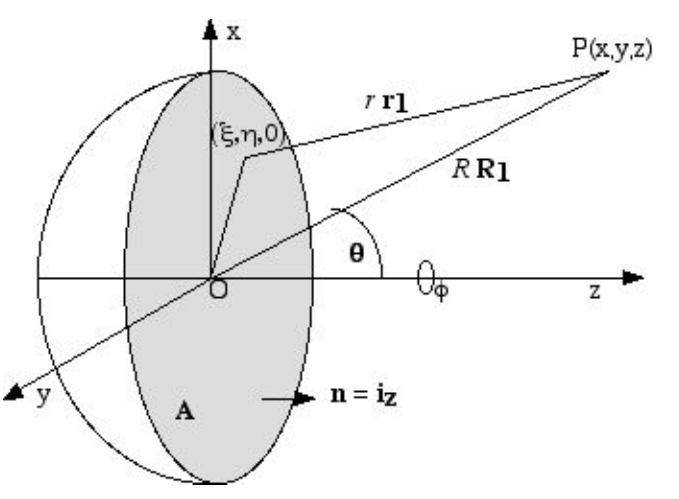
\includegraphics[width=0.5\textwidth]{images/antenna_holo.png}
    \caption{Geometry, parameters and variables used in the mathematical description.}
    \label{fig:antenna_holo}
\end{figure}


To simplify the problem some assumptions are commonly used:
\begin{enumerate}
    \item $\frac{1}{r} << k$
    \item $\frac{1}{r} \sim \frac{1}{R}$. This is not valid for the phase terms (ie the ones inside the bracket and in the exponential).
    \item  The term $\hat{z}\cdot r_1$ can be replaced by $\hat{z}\cdot R = \cos(\theta)$
    \item The term $\hat{z}\cdot \hat{s}$ represent the deviation from the uniform phase over the aperture. If the deviation is small the term can be considered to be 1.
\end{enumerate}

With all these assumptions the equation \ref{eq:holo_general} is transformed into equation \ref{eq:holo_assumptions}, where we defined $r= \sqrt{(x-\xi)^2+(y-\eta)^2+z^2}$.

\begin{equation}
f(x,y,z) = \frac{i}{2\lambda R}\int F(\xi,\eta)[\cos(\theta)+1]e^{ikr}d\eta d\xi
    \label{eq:holo_assumptions}
\end{equation}


\subsection{Far field approximation}
In the far field assumption, R tends to infinity, $R_1$ and $r_1$ are parallel then you could express $r=R-(u\xi+v\eta)$ and for a high gain antenna the interesting region is confined to small values of $\theta$ so we can  use $\cos(\theta)=1$. Then,  the equation \ref{holo_assumptions} is approximated to \ref{eq:holo_fourier}, which is a 2D Fourier transform in the aperture. So, with a given aperture distribution we are able to compute the far field using a Fourier transform. 


\begin{equation}
    f(u,v) = \frac{i}{\lambda}\frac{e^{-ikR}}{R} \int F(\xi,\eta)e^{-ik(\xi u+\eta v)} d\xi d\eta
    \label{eq:holo_fourier}
\end{equation}


The opposite is also true, we are able to compute the fields at the aperture if we measure the beam pattern. If we do that we would obtain a complex aperture $F(\xi, \eta)=A(\xi, \eta)$ and we can compute the surface errors related with the aperture phase with the equation \ref{eq:aperture2surface}. Where $\epsilon_n$ is the error normal to the surface and $F$ is the foci of the antenna. If we disregard the geometry the error is given by the Ruze formula shown in \ref{eq:ruze}

\begin{equation}
    \epsilon_n(\xi,\eta) = \frac{\lambda}{4\pi} \phi(\xi,\eta)\sqrt{1+\frac{\xi^2+\eta^2}{4F^2}}
    \label{eq:aperture2surface}
\end{equation}


\begin{equation}
    \phi = \frac{4\pi}{\lambda}\epsilon
    \label{eq:ruze}
\end{equation}


These ideas are the fundamental building blocks for the holography method to adjust an antenna:
\begin{enumerate}
    \item Make an Beam map measurement, obtaining the magnitude and phase of the signal. Typically this is done using a second antenna that is being used as reference.
    \item Compute the aperture distribution using the Fourier transform relation.
    \item Compute the surface errors on the antenna and calculate the adjustment of the panels.
\end{enumerate}


\subsection{Nearfield effects}
In this case we need to consider the phase variation in the aperture, ie the exponential terms cannot be simplified leading to a Fresnel diffraction integral shown in \ref{eq:holo_fresnel}.


\begin{equation}
    \frac{i}{\lambda}\frac{e^{ikR}}{R} \int F(\xi,\eta) exp\left(ik\left[-(u\xi+v\eta)+\frac{\xi^2+\eta^2}{2R}\right]\right)d\xi d\eta
    \label{eq:holo_fresnel}
\end{equation}


 In this case the approximation used is : $r \approx R-(u\xi+v\eta)+\delta p_1(\xi,\eta)+\epsilon$, where $\delta p_1$ contains terms that does not depends on the integration variables as shown in equations \ref{eq:holo_p1} and \ref{eq:holo_p2}.

\begin{equation}
    \delta p_1(\xi,\eta) = \frac{\xi^2+\eta^2}{2R}+\frac{(\xi^2+\eta^2)^2}{8R^3} \\
    \label{eq:holo_p1}
\end{equation}
\begin{equation}
    \epsilon = -\frac{(u\xi+v\eta)^2}{2R}+\frac{(\xi^2+\eta^2)(u\xi+v\eta)}{2R^2}
    \label{eq:holo_epsilon}
\end{equation}



To account the defocus of the telescope another term is added to $\delta p_1$, shown in the equation \ref{eq:holo_p2} where $f$ is the focal distance of the antenna and $\delta f$  is the variation of such distance.

\begin{equation}
    \delta p_2(\xi, \eta) = (\xi^2+\eta^2+(f-\frac{\xi^2+\eta^2}{4f}+\delta f)^2)^{1/2} - (f+\frac{\xi^2+\eta^2}{4f}+\delta f)
    \label{eq:holo_p2}
\end{equation}



With all these approximation the relation between the beam pattern and the aperture can be written as equation \ref{eq:holo_nearfield}, which for us is the most important equation for us.


\begin{equation}
    \boxed{ F(\xi, \eta) = \frac{i}{\lambda}\frac{e^{-ikR}}{R} exp\left(-ik[\delta p_1(\xi,\eta)+\delta p_2(\xi, \eta)]\right) \int f(u,v)exp\left(ik(u\xi+v\eta)\right)e^{-ik\epsilon} }
    \label{eq:holo_nearfield}
\end{equation}


The term $\epsilon$ can be expanded in a Taylor serie as shown in the equation \ref{eq:holo_taylor}. Depending on the accuracy that you need to met, when solving the equation \ref{eq:holo_nearfield} you can neglect some high order terms. Its good to note that the first term of the resulting equation recovers the Fourier transform relation, while the rest of the terms are modifications of the field that dissapears when $r$ is large enough.

\begin{equation}
    e^{-ik\epsilon} \approx 1-ik\epsilon = 1-ik\left[ u \frac{\xi(\xi^2+\eta^2)}{2R^2} + v \frac{\eta(\xi^2
+\eta^2)}{2R^2}-u^2\frac{\xi^2}{2R}-v^2\frac{\eta^2}{2R}-uv\frac{\xi\eta}{R} \right]
    \label{eq:holo_taylor}
\end{equation}



\subsection{Zernike polynomials}
Since the final goal of a radio holography measurement is to compute the adjustment of the panels that forms the primary reflector, we need to isolate the errors that comes from the single panel position and rule out the large scale errors that are present in the telescope, like for example optical aberrations. 


Zermike polynomials are a sequence of orthogonal polynomials on the unitary disk. They are used to describe different types of aberrations on optics. 
One advantage of the zernike polynomials is that they can be normalized, so the value of each component is proportional to the overall effect on the surface error.



The Zernike polynomils in the unit circle can be represented by the equations \ref{eq:zernike_eq} and \ref{eq:zernike_radial}. In the figure \ref{fig:zernike_pols} the first Zernike terms are shown.


\begin{equation}
    U_{n}^{m}(\rho, \theta) = \begin{cases}
        R_{n}^{m}(\rho)\cos(m \theta) & m \ge 0 \\
        R_{n}^{m}(\rho)\sin(m \theta) & m < 0
    \end{cases}
    \label{eq:zernike_eq}
\end{equation}

\begin{equation}
    R_{n}^{m}(\rho) = \frac{1}{\left(\frac{n-m}{2} \right) \rho^m} \left( \frac{d}{d(\rho^2)} \right)^{\frac{n-m}{2}} \left[ \left(\rho^2 \right)^{\frac{n+m}{2}} \left( \rho^2-1 \right)^{\frac{n-m}{2}} \right]
    \label{eq:zernike_radial}
\end{equation}



\begin{figure}
    \centering
    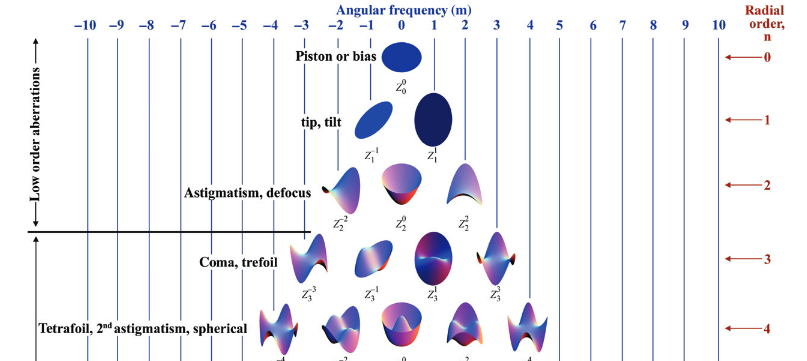
\includegraphics[width=0.9\textwidth]{images/zernike_pols.png}
    \caption{First Zernike polynomials.}
    \label{fig:zernike_pols}
\end{figure}















\end{document}
